\subsection{Bewertung der Testergebnisse}
Nach dem durchlaufen der Tests wurden die Ergebnisse ananlysiert und bewertet. Dabei wurde nicht nur die Genauigkeit der Gipfelerkennung bewertet, sondern auch die durchschnittlichen und extremen Abweichungen für Position, Höhe, Prominenz und Dominanz, sowie die Laufzeit. Dabei werden zunächst alle Test-Szenarien einzeln bewertet und anschließend die Ergebnisse zusammengefasst. Dabei wurden zur besseren Vergleichbarkeit alle Tests mit einer Boder width von 50px ausgeführt. \todo{border with auf deutsch formulieren} Außerdem wurde bei allen Test mit einer minimalen orographischen Dominanz von 0\% gerechnet. Letzteres hat den Grund, dass die orographische Dominanz aus der Prominenz und der Höhe berechnet werden kann. Daher ist es einfacher zum testen dieser Funktion keine Feldtests durchgeführen, sondern einfache Unittests zu schreiben. \todo{verweis auf unittests}

\subsubsection{Wetterstein-Tests}
Im Wettersteingebirge und Umland wurden mit dem Algorithmus alle Berge mit einer minimalen Höhe von 0m, Prominenz von über 500m und Dominanz von minimal 2km gesucht. Diese Werte wurden gewählt, damit die Zahl der zu untersuchenden Gipfel nicht zu groß ausfällt. In diesem Test wurden 95\% der realen Gipfel auf 1000m korrekt erkannt (Precision) und 68\% der gefundenen Gipfel waren in 1000m um einen realen Gipfel, der den Kriterien entsprach (Sensitivity). \todo{abgleich wirklich geleich emtriken wie in 4.2} Bei einem Vergleichsbereich von 100m werden noch 60\% der Gipfel richtig erkannt. Auf den Pixel genau (ca. 65m) werden nur 55\% der Gipfel erkannt. Die Restlichen Metriken sind hier in einer Tabelle zu finden: \todo{diese überleitung umformulieren}

\begin{table}[htbp]
\centering
\caption{Metriken (scope = 100\,m)}
\label{tab:metrics_100m_circular}
\begin{tabular}{|l|r|}
\hline
Metrik & Wert \\
\hline
Precision & 0.60 \\
\hline
Sensitivity & 0.43 \\
\hline
F1-Score & 0.50 \\
\hline
Durchschnittlicher Positionsfehler (m) & 30.83 \\
\hline
Durchschnittlicher x-Fehler (m) & 23.35 \\
\hline
Durchschnittlicher y-Fehler (m) & 17.44 \\
\hline
Durchschnittlicher Höhenfehler (m) & 26.83 \\
\hline
Durchschnittlicher Dominanzfehler (m) & 641.77 \\
\hline
Durchschnittlicher Prominenzfehler (m) & 97.33 \\
\hline
\end{tabular}
\end{table}

\todo{matching areas auf pixelwidth/2 bei pixelgenauc und rest auf 100m und 1000m  circular setzen}
\begin{table}[htbp]
\centering
\caption{Metriken (scope = 65.15651688191356\,m)}
\label{tab:metrics_65m_square}
\begin{tabular}{|l|r|}
\hline
Metrik & Wert \\
\hline
Precision & 0.55 \\
\hline
Sensitivity & 0.39 \\
\hline
F1-Score & 0.46 \\
\hline
Durchschnittlicher Positionsfehler (m) & 26.06 \\
\hline
Durchschnittlicher x-Fehler (m) & 21.39 \\
\hline
Durchschnittlicher y-Fehler (m) & 12.65 \\
\hline
Durchschnittlicher Höhenfehler (m) & 26 \\
\hline
Durchschnittlicher Dominanzfehler (m) & 677.45 \\
\hline
Durchschnittlicher Prominenzfehler (m) & 91.82 \\
\hline
\end{tabular}
\end{table}

\begin{table}[htbp]
\centering
\caption{Metriken (scope = 1000\,m)}
\label{tab:metrics_1000m_circular}
\begin{tabular}{|l|r|}
\hline
Metrik & Wert \\
\hline
Präzision & 0.95 \\
\hline
Sensitivität & 0.68 \\
\hline
F1-Score & 0.79 \\
\hline
Durchschnittlicher Positionsfehler (m) & 149.88 \\
\hline
Durchschnittlicher x-Fehler (m) & 130.65 \\
\hline
Durchschnittlicher y-Fehler (m) & 51.19 \\
\hline
Durchschnittlicher Höhenfehler (m) & 32.47 \\
\hline
Durchschnittlicher Dominanzfehler (m) & 1040.35 \\
\hline
Durchschnittlicher Prominenzfehler (m) & 98.58 \\
\hline
\end{tabular}
\end{table}

\todo{problem solstein}

In diesen Allgemeinen Testergenissen ist gut zu erkennen, dass der Tester weniger Probleme damit hat Gipfel zu erkennen, sondern deren Prominenz und Dominanz richtig zu bestimmen. Das zeigt sich in den für die gewählten Schwellenwerte hohen durchscnittlichen Prominenz und Dominanz. Um nun genauer zu erkennen, was für die Abweichungen verantwortlich ist, müssen die einzelnen Werte untersucht werden. Dabei fällt auf, dass die meisten Berge eine unerwartet hohe Dominanzabweichung haben. Dabei gibt es auch ein paar Gipfel, die besonders hohe oder niedrige Abweichungen haben. Diese sind für die Bestimmung der Fehlerursache wichtig. Der Gipfel mit der höchsten Abweichung ist die Birkkarspitze (11,5km) und der Gipfel mit der niedrigsten ist der Hochplattig (36m). Eine höhere Abweichung der Dominanz vom Realwert lässt sich bei der Birkkarspitze zwar alleine durch die Hohe Dominanz von 33km erklären, aber 11,5km ist dennoch zu hoch um nicht auf einen Fehler im Höhenmodell oder Algorithmus hinzudeuten. Um das Problem besser einordnen zu können, werden die Gipfel und ihre Possition, sowie nächst höheren Punkte miteinander verglichen. Das folgende Diagramm \ref{fig:Dominanz_von_Wetterstein} zeigt den Kartenbereich und vier Gipfel die so aufbereitet wurden. 

\begin{figure}[h] % h=here, t=top, b=bottom, p=page
    \centering
    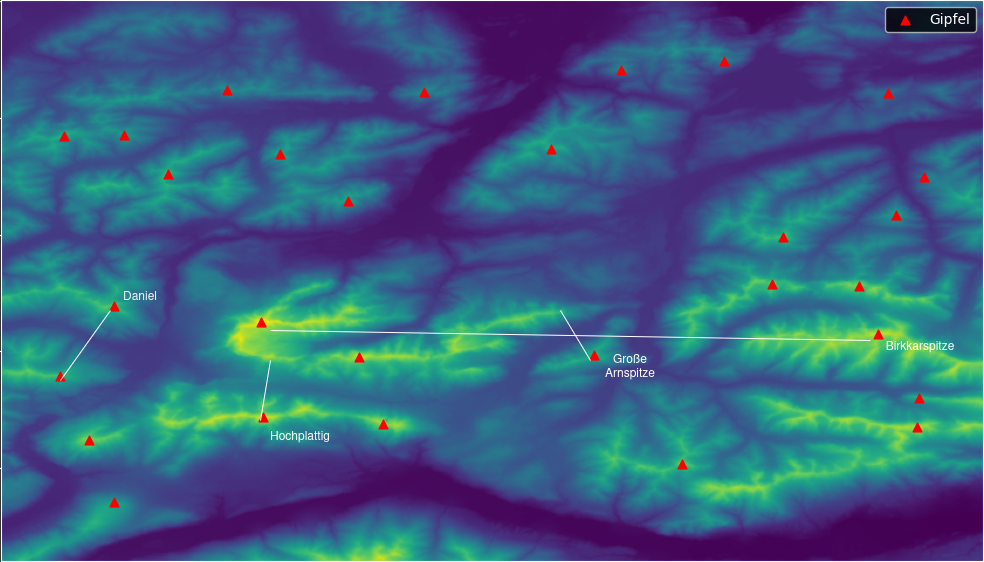
\includegraphics[width=1.0\textwidth]{Diagramms/Dominenz_Wetterstein.drawio.png}
    \caption{Dominanz von Daniel, Birkkarspitze, Hochplattig und Große Arnspitze}
    \label{fig:Dominanz_von_Wetterstein}
\end{figure}

Zusätzlich sind die relativen Fehler der Dominanzen in dem Diagramm \ref{tab:relativer_fehler_Wetterstein} zu sehen. Hieran ist gut zu erkennen, dass der Hochplattig der einzige Berg ist, desen Dominanz nur in Y-Richtung bestimmt wurde. \todo{schlussfoldern, das berechnung der Distanz Müll}

\begin{table}[htbp]
\centering
\caption{Relative Fehler pro Gipfel}
\label{tab:relativer_fehler_Wetterstein}
\begin{tabular}{|l|r|}
\hline
Gipfel & Wert (\%) \\
\hline
Birkkarspitze & 34,84\%  \\
\hline
Hochplattig & 0,6\% \\
\hline
Daniel & 36,0\% \\
\hline
Große Arnspitze & 16,9\% \\
\hline
\end{tabular}
\end{table}

Ein anderes Problem ist, dass der Algorithmus Gipfel erkennt, die in Realität nicht existieren. Das passiert nur in der Nähe des Kartenrandes. Das liegt daran, dass kleine Erhebungen am Hang eines Berges nahe des Kartenrandes nicht als Gipfel ausgeschlossen  werden können. In diesem Fall wird ihnen der Hang des gesammten Berges bei der Prominenzberechnung angerechent. \todo{diagram mit Zylinder oder berg und dann ne border durch/ höhenlinien an border} Um dies zu verhindern wurde bereits die \textit{border width} eingeführt. Diese scheint aber nicht richtig zu funktionieren, die Randwertfehler nun am Rand der \textit{border width} auftretten.

\todo{das border width problem diagramm}

Der Algorithmus erkennt einzelne Gipfel nicht als Gipfel. In diesem Test-Szenario ist das der kleine Solstein bei Innsbruck. Der Grund hierfür ist, dass seine Prominenz als unter 500m vorhergesagt wird, obwohl sie bei 517m liegt. Dieses Problem lässt sich auf die Kartenqualität zurückführen. 

Wenn ein Gipfel in dem Vergleichsbereich um einen realen Gipfel liegt, heißt das nicht, dass der Algorithmus den Gipfel erkennt. Das wird bei der Birkkarspitze erkenntlich, wo der Algorithmus die mittlere Ödkarspitze als Gipfel erkannt hat, die eigentliche Birkkarspitze nicht. Dieser Fehler kann mit der genauigkeit der Karte erklärt werden. 

\subsubsection{Feldberg-Test}
Beim Feldberg-Test wurden mit dem Algorithmus alle Berge mit einer minimalen Höhe von 0m, Prominenz von über 100m und Dominanz von minimal 200m gesucht. Diese Werte wurden gewählt, damit die Zahl der zu untersuchenden Gipfel auf diesem kleineren Kartenasuschnitt nicht zu gering wird. Mit diesen Parametern wurden 91\% der realen Gipfel auf 100m korrekt erkannt und 67\% der gefunden Gipfel waren reale Gipfel. Dies zeigt ein ähnliches Bild, wie auch schon der Wetterstein-Test. Der Algorithmus findet zwar die meisten Gipfel, findet jedoch auch zusätzliche Gipfel nahe des Randes, die keinen realen Gipfel entsprechen. Anders als beim Wetterstein-Test bestimmt der Algorithmus beim Feldbergtest nur 18\% der Gipfel auf den Pixel genau. Dies kann durch die kleinere Rastergröße von 10m und die Genauigkeit der Realwerte erklärt werden. Weitere Metriken der Tests sind in den Tabellen \ref{tab:metrics_Feldberg_5m} und \ref{tab:metrics_Felbgerg_100m} enthalten.

\begin{table}[htbp]
\centering
\caption{Metriken (scope = 5\,m)}
\label{tab:metrics_Feldberg_5m}
\begin{tabular}{|l|r|}
\hline
Metrik & Wert \\
\hline
Präzision & 0.18 \\
\hline
Sensitivität & 0.13 \\
\hline
F1-Score & 0.15 \\
\hline
Durchschnittlicher Positionsfehler (m) & 7.11 \\
\hline
Durchschnittlicher x-Fehler (m) & 4.84 \\
\hline
Durchschnittlicher y-Fehler (m) & 5.14 \\
\hline
Durchschnittlicher Höhenfehler (m) & 5.0 \\
\hline
Durchschnittlicher Dominanzfehler (m) & 30.8 \\
\hline
Durchschnittlicher Prominenzfehler (m) & 1.5 \\
\hline
\end{tabular}
\end{table}

\begin{table}[htbp]
\centering
\caption{Metriken (scope = 100\,m)}
\label{tab:metrics_Felbgerg_100m}
\begin{tabular}{|l|r|}
\hline
Metrik & Wert \\
\hline
Präzision & 0.91 \\
\hline
Sensitivität & 0.67 \\
\hline
F1-Score & 0.77 \\
\hline
Durchschnittlicher Positionsfehler (m) & 30.86 \\
\hline
Durchschnittlicher x-Fehler (m) & 20.15 \\
\hline
Durchschnittlicher y-Fehler (m) & 19.91 \\
\hline
Durchschnittlicher Höhenfehler (m) & 2.1 \\
\hline
Durchschnittlicher Dominanzfehler (m) & 21.15 \\
\hline
Durchschnittlicher Prominenzfehler (m) & 3.3 \\
\hline
\end{tabular}
\end{table}

An diesem Testfall ist gut zu erkennen, dass die Karten des Vermessungsamtes Baden Württemberg genauer sind als die öffentlich zugänglichen Daten des Copernikusprogramms. Dies spiegelt sich in den geringeren Höhen- sowie Positionsfehlern wieder. Außerdem zeigen diese Tests, dass der Algorithmus die Gipfel nicht in eine bestimmte Richtung genauer oder ungenauer bestimmt, anders als es die Testdaten des Wettersteingebirge vermuten lassen. 
\todo{geringe Dominanz sowie Prominenzabweichungen}

\subsubsection{Südschwarzwald-Test}
Beim Südschwarzwald-Test wurden mit dem Algorithmus alle Berge mit einer minimalen Höhe von 0m, Prominenz von über 100m und Dominanz von minimal 2000m gesucht. Dabei wurden wie bei den letzten Tests auf 1000m Genauigkeit über 90\% der Gipfel richtig bestimmt und 79\% der gefundenen Gipfel waren real. Die genauen Testergebnisse können in den Tabellen \ref{tab:metrics_Blackforrest_1000m}, \ref{tab:metrics_Blackforrest_100m} und \ref{tab:metrics_Blackforrest_15m} abgelesen werden. Dabei fällt auf, dass die Höhenungenauigkeiten ungefähr einem Drittel des Wetterstein-Tests entsprechen. Das bedeutet, dass es wahrscheinlcih ist, dass das verringern der Auflösung einen Einfluss auf die Ergebnisse hatte. Zudem kann erkannt werden, dass mit schlechterer Auflösung die Dominanzen ungenauer werden. Es kann beobachtet werden, dass der Prominenzfehler ungefähr dem doppelten Höhenfehler entspricht.

\begin{table}[htbp]
\centering
\caption{Metriken (scope = 15\,m)}
\label{tab:metrics_Blackforrest_15m}
\begin{tabular}{|l|r|}
\hline
Metrik & Wert \\
\hline
Präzision & 0.28 \\
\hline
Sensitivität & 0.23 \\
\hline
F1-Score & 0.25 \\
\hline
Durchschnittlicher Positionsfehler (m) & 5.26 \\
\hline
Durchschnittlicher x-Fehler (m) & 3.95 \\
\hline
Durchschnittlicher y-Fehler (m) & 2.27 \\
\hline
Durchschnittlicher Höhenfehler (m) & 7.7 \\
\hline
Durchschnittlicher Dominanzfehler (m) & 1333.92 \\
\hline
Durchschnittlicher Prominenzfehler (m) & 14.2 \\
\hline
\end{tabular}
\end{table}

\begin{table}[htbp]
\centering
\caption{Metriken (scope = 100\,m)}
\label{tab:metrics_Blackforrest_100m}
\begin{tabular}{|l|r|}
\hline
Metrik & Wert \\
\hline
Präzision & 0.72 \\
\hline
Sensitivität & 0.6 \\
\hline
F1-Score & 0.66 \\
\hline
Durchschnittlicher Positionsfehler (m) & 35 \\
\hline
Durchschnittlicher x-Fehler (m) & 22.12 \\
\hline
Durchschnittlicher y-Fehler (m) & 10.23 \\
\hline
Durchschnittlicher Höhenfehler (m) & 10.23 \\
\hline
Durchschnittlicher Dominanzfehler (m) & 997.33 \\
\hline
Durchschnittlicher Prominenzfehler (m) & 45.35 \\
\hline
\end{tabular}
\end{table}

\begin{table}[htbp]
\centering
\caption{Metriken (scope = 1000\,m)}
\label{tab:metrics_Blackforrest_1000m}
\begin{tabular}{|l|r|}
\hline
Metrik & Wert \\
\hline
Präzision & 0.94 \\
\hline
Sensitivität & 0.79 \\
\hline
F1-Score & 0.86 \\
\hline
Durchschnittlicher Positionsfehler (m) & 82.19 \\
\hline
Durchschnittlicher x-Fehler (m) & 45.58 \\
\hline
Durchschnittlicher y-Fehler (m) & 61.71 \\
\hline
Durchschnittlicher Höhenfehler (m) & 9.79 \\
\hline
Durchschnittlicher Dominanzfehler (m) & 893.68 \\
\hline
Durchschnittlicher Prominenzfehler (m) & 40.56 \\
\hline
\end{tabular}
\end{table}

\todo{Laufzeittests in 5 zu finden}